%%%%%%%%%%%%%%%%%%%%%%%%%%%%%%%%%%%%%%%%%%%%%%%%%%%%%%%%%%%%%%%%%%%%%%%%%%%%%%%%%%%%%%%
%%%%%%%%%%%%%%%%%%%%%%%%%%%%%%%%%%%%%%%%%%%%%%%%%%%%%%%%%%%%%%%%%%%%%%%%%%%%%%%%%%%%%%%
% 
% This top part of the document is called the 'preamble'.  Modify it with caution!
%
% The real document starts below where it says 'The main document starts here'.

\documentclass[12pt]{article}

\usepackage{amssymb,amsmath,amsthm}
\usepackage[top=1in, bottom=1in, left=1.25in, right=1.25in]{geometry}
\usepackage{fancyhdr}
\usepackage{enumerate}
\usepackage{hieroglf}
\usepackage{times,txfonts}
\usepackage{graphicx}
\usepackage{float}

% Comment the following line to use TeX's default font of Computer Modern.
\usepackage{times,txfonts}

\newtheoremstyle{homework}% name of the style to be used
  {18pt}% measure of space to leave above the theorem. E.g.: 3pt
  {12pt}% measure of space to leave below the theorem. E.g.: 3pt
  {}% name of font to use in the body of the theorem
  {}% measure of space to indent
  {\bfseries}% name of head font
  {:}% punctuation between head and body
  {2ex}% space after theorem head; " " = normal interword space
  {}% Manually specify head
\theoremstyle{homework} 

% Set up an Exercise environment and a Solution label.
\newtheorem*{exercisecore}{Exercise \@currentlabel}
\newenvironment{exercise}[1]
{\def\@currentlabel{#1}\exercisecore}
{\endexercisecore}

\newcommand{\localhead}[1]{\par\smallskip\noindent\textbf{#1}\nobreak\\}%
\newcommand\solution{\localhead{Solution:}}

%%%%%%%%%%%%%%%%%%%%%%%%%%%%%%%%%%%%%%%%%%%%%%%%%%%%%%%%%%%%%%%%%%%%%%%%
%
% Stuff for getting the name/document date/title across the header
\makeatletter
\RequirePackage{fancyhdr}
\pagestyle{fancy}
\fancyfoot[C]{\ifnum \value{page} > 1\relax\thepage\fi}
\fancyhead[L]{\ifx\@doclabel\@empty\else\@doclabel\fi}
\fancyhead[C]{\ifx\@docdate\@empty\else\@docdate\fi}
\fancyhead[R]{\ifx\@docauthor\@empty\else\@docauthor\fi}
\headheight 15pt

\def\doclabel#1{\gdef\@doclabel{#1}}
\doclabel{Use {\tt\textbackslash doclabel\{MY LABEL\}}.}
\def\docdate#1{\gdef\@docdate{#1}}
\docdate{Use {\tt\textbackslash docdate\{MY DATE\}}.}
\def\docauthor#1{\gdef\@docauthor{#1}}
\docauthor{Use {\tt\textbackslash docauthor\{MY NAME\}}.}
\makeatother

% Shortcuts for blackboard bold number sets (reals, integers, etc.)
\newcommand{\Reals}{\ensuremath{\mathbb R}}
\newcommand{\IRats}{\ensuremath{\mathbb I}}
\newcommand{\Nats}{\ensuremath{\mathbb N}}
\newcommand{\Ints}{\ensuremath{\mathbb Z}}
\newcommand{\Rats}{\ensuremath{\mathbb Q}}
\newcommand{\Cplx}{\ensuremath{\mathbb C}}
%% Some equivalents that some people may prefer.
\let\RR\Reals
\let\NN\Nats
\let\II\Ints
\let\CC\Cplx


\doclabel{Math F316}
\docauthor{Stefano Fochesatto}
\docdate{\today}% DATE READING SENTENCES ARE DUE GOES HERE


%%%% Main document starts here.

\begin{document}

\section*{4.1-4.2}

\begin{description}
\item[Enlightening summary \#1:]
 Section 4.1 describes the founding of the city of Alexandria by Alexander the Great and later carried out by Ptolemy. The followers of Ptolemy
 dedicated themselves to making Alexandria the center of intellectual life, by founding the Museum and the Alexandrian Library. The text also goes on to 
 describe the heavy-handed methods by which the Alexandrian library attained their manuscripts. The Museum produced and incredible amount of distinguished scholars, with 
 Euclid being perhaps the most influential. The rest of the section recounts Euclid's life and writings. Personally I love the story about King Ptolemy asking for a shorter way to
 learn geometry, to which Euclid responded with  "There is no royal road to geometry". 
 
\item[Enlightening summary \#2:] 
 Continuing the thread, Section 4.2 goes more in depth on the work from "The Geometer". The text explains the necessity 
 for Euclid's Postulates and even emphasizes the controversy behind Euclid's parallel postulate which would later come to a head with the formulation of
 non-Euclidean geometry. We also see criticisms of Euclid's Elements with the main objection being the lack of rigor, and tacit assumptions that are omitted from 
 the postulates. The prime examples being Euclid's use of "superposition" and his failure to ensure the continuity of lines and circles. The rest of the section gives a rundown of
 some of the propositions from Book I. The text also discusses Book II, which focuses on geometric algebra, with the biggest takeaway being that it allowed the Greeks to solve quadratic 
 equations without irrational numbers. 


\item[Interesting:] I really really like Micheal Stifel's description of irrational numbers as being hidden in a "cloud of infinity". I also interested in
the section that explains why certain definitions in a logical system must remain undefined. Thinking back to geometry class last semester,
it seems like trying to prove Euclid's parallel postulate is a right of passage for anyone interested in geometry.                                                                                                 
 
 

\item[Confusing:] While I am aware that Greek geometric algebra was handicapped by only being able to express linear and quadratic equations, how is it any different from our symbolic representation?
Although it may be "cumbersome" and "overwhelming" in the end a line segment that represents $\sqrt{2}$ is just as meaningful as our notation. Furthermore I'm fairly certain I've seen the Babylonian 
complete the square algorithm applied to cubic functions, did they not experiment in 3-dimensions?
\begin{center}
  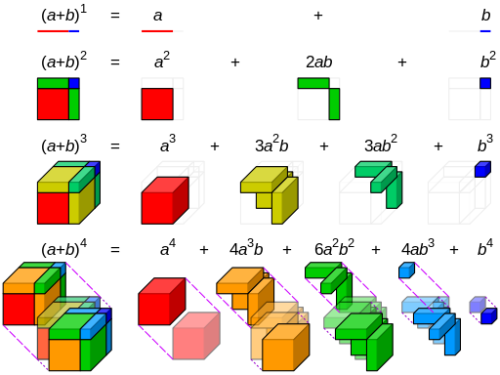
\includegraphics[width = .75\textwidth]{solve.png}        
\end{center}

\end{description}
\end{document}
